\documentclass[10pt]{IETBook}
\usepackage{graphicx}
\usepackage{epsfig}
\usepackage{graphics}
\usepackage{booktabs}
\usepackage{cite}
\usepackage{array}
\usepackage{longtable}

\begin{document}

%For RH Book title
\rhbooktitle{Information and Communication Technologies for Humanitarian Services}

\markboth{Information and Communication Technologies for Humanitarian Services}{ICT for Humanitarian Services}

\cauthor{Arvind W. Kiwelekar, Sanil Gandhi, Laxaman D. Netak\thanks{Department of Computer Engineering, Dr. Babasaheb Ambedkar Technological University Lonere-402103 Raigad(MS) India}}


\chapter{Use-cases of Blockchain Technology for Humanitarian Engineering}

\section*{Abstract} Humanitarian Engineers need innovative methods to make
technological interventions for solving  societal problems. 
The emerging Blockchain technology has the enormous potential to provide effective interventions in various developmental sectors including Agriculture, Education, Health, and Transportation. 
In these sectors, mediators, either in the form of individuals or organizations, are seen as one of the impediments for developmental work. 
The Blockchain technology facilitates peer-to-peer business transactions without any mediators.
Thus, the Blockchain technology is emerging as an alternative to conventional mediator-centred solutions adopting client-server based Internet technologies.

The Blockchain technology can be combined with other technologies to address domain specific challenges. 
For example, the combination of Blockchain technology and Internet-of-Thing (IoT) has the potential to monitor usage of scarce resources such as the level of ground-water and amount of energy consumption. 
The combination of Radio Frequency Identification (RFID) and Blockchain technology assists in ascertaining the provenance of agricultural and handicraft products thus avoiding the exploitation of original producers from  duplicate or hackneyed producers.

The aims of this Chapter are threefold. Firstly, it describes the primary building blocks of Blockchain technology. Secondly, it illustrates various use-case scenarios of Blockchain technology combined with RFID, IoT and Artificial Intelligence in the field of Agriculture, Energy consumption, monitoring of usages of natural resources, the provenance of natural and handicrafts products. 
Thirdly, it evaluates the existing platforms supporting Blockchain-based application development.


\section{Humanitarian Engineering: An Example}

The goal of Humanitarian Engineering is to help underprivileged and marginalized people.  
It does so by designing and implementing technology-based solutions to address the challenges faced by such people. The {\em Jaipur foot} \cite{arya2008jaipur} is one of the best examples of humanitarian engineering products. The Jaipur foot is an artificial leg designed to help people with below-knee leg amputation. It uses a new material of that time called {\em polyurethane} to develop near-natural but artificial leg. Since the last fifty years, the Jaipur foot has been assisting thousands of physically challenged people to compete with ordinary people, bringing a smile on their faces. Durability, flexibility and convenience of use are some of the critical factors behind the successful and widespread use of Jaipur foot which was the result of innovative use of material technology.

The example of {\em Jaipur foot} illustrates two significant aspects of humanitarian engineering. First one is the use of technology, i.e. material technology in case of Jaipur foot and the second one is relieving pain or grief of underprivileged people.

The focus of this chapter is on the Blockchain Technology, one of the emerging Information and Communication 
Technologies. The objective of this chapter is to illustrate how Blockchain technology has promising applications to address diverse needs of various developmental sectors as envisaged by UN sustainable development program. 

\section{A Framework for understanding Humanitarian Engineering}
Before delving into details of technological alternatives for realizing humanitarian engineering let us develop a framework to understand the dynamics of humanitarian engineering as a discipline. The three main pillars of humanitarian engineering are: (1) Stakeholders (2) 
Goals (3) Sectors for humanitarian engineering.

\begin{table}[t]
\begin{center}
\begin{tabular}{|p{0.15in}|p{0.66in}| p{3.2in}|}
\hline
Sr. No. & Development \newline Agencies & Activities \\ \hline 
1 & UNDP & United Nations Development Program (UNDP) is one of the subunits of the United Nations headquartered in New York City. The primary role of the UNDP is to formulate policies, set priorities, and sponsor development programs to address the challenges faced by humanity. It does so by proactively working with all the member nations of United Nations Organizations (UNO).\cite{mccall2013undp} \\ \hline

2 & UNWFP & United Nations World Food Program (UNWFP) is a branch of UNO raising the war against hunger and malnutrition. It provides food assistance to member countries so that the nutritional needs of the people leaving in poverty. It aims to reduce child mortality, improve maternal health and to fight against diseases. \cite{fao2015wfp}\\ \hline
     
3 & WHO & World Health Organization (WHO) is a subsidiary of UNO dealing with matters of public health at the international level. It articulates policies for ensuring the highest possible health for individuals by identifying social and economic factors affecting health. It closely works with national government agencies and monitors the effective implementation of health policies. \cite{world2002traditional}\\ \hline 
\end{tabular}
\centering{\caption{\bf International Development Agencies and Their Role}} 
\label{international}
\end{center}
\end{table}

\subsection{Stakeholders for Humanitarian Engineering}
The main stakeholders for humanitarian engineering projects are the people and organizations that play critical role in the development of underprivileged communities.These are also known as {\em development agencies}. These agencies operate at different geographical levels from global to local level.

The first kinds of development agencies are {\em international development agencies}. Their primary function is to address the problems faced by humankind. These agencies set the agenda
for development programs, identify the problems faced by humankind, monitor and evaluate the performance of development programs, collect data and evidences to study the impact of development programs and to fund the developmental activities in various countries. 

The role three leading international development agencies are described in Table \ref{international}.  
13

Besides this,  World Bank and Asian Development Banks (ADB) are some of the other international development agencies which sponsor developmental projects.

Many countries in the world have development agencies at the national level to formulate country-specific development policies, align it with policies formulated by UNDP, and implement developmental projects. For example in India, National Initiative for Transforming India (NITI) Aayog, is one such organization.

Also, there are some regional development agencies whose primary role is to implement the developmental projects in coordination with national and international agencies. In a few countries, universities and academic Institutes are slowly emerging as a regional knowledge centre to provide information necessary to get insights about the local developmental needs \cite{uni}.


\subsection{Sustainable Development Goals}
The Sustainable Development Goals (SDG) capture the expectations and aspirations of people to live in a prosperous society without compromising on the needs of future generations. These SDGs are a set of ambitious goals put forward by the UN in the Year 2015 for the entire development of humanity \cite{assembly2015sustainable,nilsson2016policy}. These set of goals are linked 
to specific targets to be achieved by the end of the year 2030. Table \ref{sdg} list out all seventeen goals categorized into five labels namely People, Prosperity, Peace, Partnership and Planet \cite{wu2018information}.

\begin{table}[!t]
	\begin{center}
		\begin{tabular}{|p{0.68in}|p{1.75in}|p{2in}| } \hline
			Category & SDGs & Description \\ \hline 
			
			{\bf People} & (SDG1) No Poverty, \newline (SDG2) Zero Hunger, \newline (SDG3) Good Health and Well-being, \newline (SDG4) Quality Education, \newline (SDG5) Gender Equality & End poverty and hunger in all their forms and dimensions, ensure all human beings can fulfill their potential in dignity, equality and healthy environment. \\ \hline   
			
			{\bf Prosperity} & (SDG8) Decent Work and Economic Growth, & Enjoy prosperous and fulfilling lives, economic, social, and technological harmonic progress \\ \hline 
			
			{\bf Peace} & (SDG10) Reducing Inequality, \newline (SDG16) Peace, Justice, and Strong Institutions & Foster peaceful, just and inclusive societies, free from fear and violence. \\ \hline 
			
			{\bf Partnership} & (SDG17) Partnerships for the Goals. & Revitalized global Partnership, participation of all countries, stakeholders and people. \\ \hline 
			
			{\bf Planet} & (SDG6) Clean Water and Sanitation, \newline (SDG7) Affordable and Clean Energy, \newline (SDG9) Industry, Innovation, and Infrastructure \newline (SDG11) Sustainable Cities and Communities,\newline (SDG12) Responsible Consumption and Production, \newline (SDG13) Climate Action, \newline (SDG14) Life Below Water, \newline(SDG15) Life On Land & Protect degradation through sustainable consumption, production, natural resource management,  stakeholders and people \\ \hline 
		\end{tabular}
		\caption{\bf Sustainable Development Goals}
		\label{sdg}
	\end{center}
\end{table}

\begin{figure}
\centering
	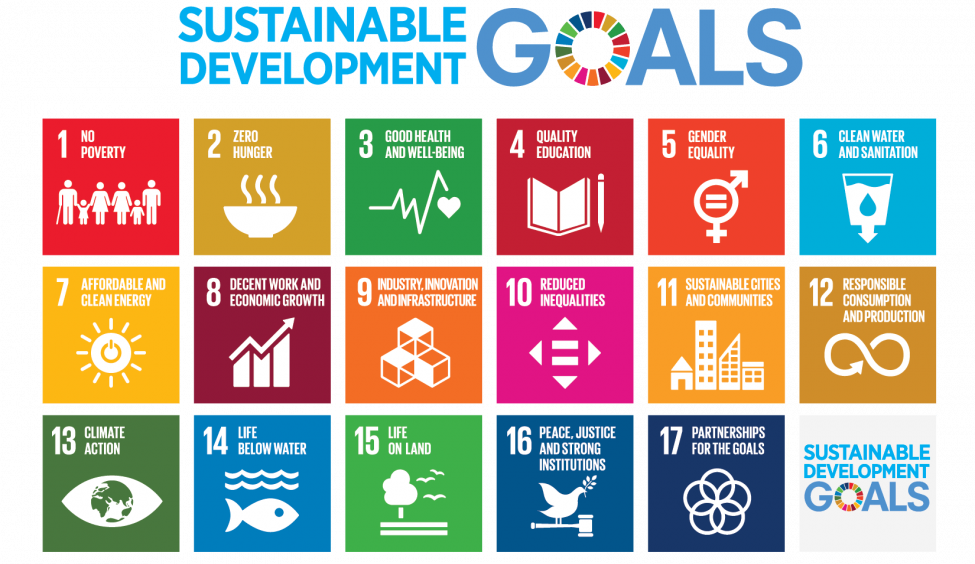
\includegraphics[width=3.5in]{SDGs}
	\caption{Sustainable Development Goals}
\end{figure}

Achieving these goals is an enormous task. Development agencies need to devise social, legal, financial and technological interventions. A development engineer responsible for technological interventions should know these SDGs so that project objectives and outcomes can be aligned with the SDGs. Knowledge of these SDGs is also essential for any engineer to become conscious about societal needs and environmental responsibilities.

\subsection{Sectors for Humanitarian Engineering}
The set of SDGs described in the last section aims for the overall development of humanity. The three main sectors which directly capture needs of human being responsible for achieving SDGs are Economical systems, Social systems and Environmental systems. However, some institutes and sectors are responsible to lay the operational and legal framework necessary for business transactions. This section reviews such business sectors responsible for achieving the target indicators set for each SDGs.

\begin{enumerate}
 \item {\bf Agriculture} The agriculture sector is the most crucial  sector for sustainable development. The SDGs like {\em End Poverty} and {\em Zero Hunger} are directly related to agricultural production. Feeding the ever growing population with sufficient food and nutrient is a huge task. As most of the rural population depends on income from agricultural produce, the goal of ending poverty is also correlated with agriculture. The sustainable agricultural 
production is constrained by factors like growing population, water shortages, declining soil fertility and climate change \cite{wu2018information}. Recently scientists have been exploring technologies such as Wireless sensor technologies\cite{culibrina2015smart} and ICT\cite{singh2015innovation} for Sustainable agricultural production.
 \item {\bf Banking and Finance}
 Banking and financial markets drive economic development. It provides capital to start new businesses. It provides various avenues for income growth and wealth accumulation \cite{rioja2004finance}. The number of banks and non-banking financial institutes present in the community is one of the indicators of economic development. Trust in financial institutes, efficient of processing business transactions(e.g., remittances, payment made to farmers on selling upon crops) diversity of financial instruments (e.g., crop insurance, loans, micro-credits) are some of the factors necessary of decent work and economic growth. Emerging technologies such as cryptocurrencies have to play a significant role in making business transactions simpler. 
 \item {\bf Education} Education brings changes in behavior. Education makes people more knowledgeable and skillful to get decent jobs. Education brings awareness about the environment, and once social responsibility. It also has an indirect impact on the health of an individual, reduction in the rate of population growth. The task providing education to all is becoming more challengable because of a shortage of trained teachers, difficulties in providing better learning experiences to students on account of a shortage of playground in urban areas and over sized classrooms. Educators are gradually adopting technologies to overcome some of these challenges.
 \item {\bf Energy} The goal of {\em affordable and clean energy} (SDG7) is directly related with
 energy sector. This sector also drives industrial development and economic growth. The demand for energy is increasing exponentially because of increasing population and wide-spread use of electro-mechanical devices to carry out routine works. Conventional energy generation methods that use natural resources such as coal and fossil fuels fails to meet this increasing energy demand. Hence use of non-conventional and renewable energy sources need to be increased on a large scale for sustainable development. In this context, it is required to provide technological solutions that would reduce energy demand, techniques for efficient energy production and replacement of conventional energy sources.\cite{lund2007renewable}
 \item {\bf E-Governance} E-government is the use of Information and Communication Technologies (ICT) into day-to-day government processes. It is aimed to bring effectiveness in administration, transparency in the services provided by the government, and increasing participation of citizens in implementing government policies. The sector of E-governance is directly linked to Goal 16 and Goal 17. This sector plays a critical role in building accountable institutes necessary for enforcing peace and justice in societies (Goal 16). It also lays the technological infrastructure necessary to strengthen partnership at the global level required to implement various SDGs (Goal 17). \cite{ndou2004government,lim2016government}
 
 \item {\bf Environment Science and Engineering}
 The policy makers formulating the developmental goals have realized the drawbacks of uncontrolled development that took place in the last century. The economic growth that pollutes air and water, that reduces the portion of forest and agricultural land, never satisfy the needs of the future generation. Hence the SDGs such as the provision of clean water and sanitation (SDG6) actions for regulating climate change (SDG13) and protecting life below water and on land (SDG14 \& SDG15) are directly linked to environmental science and engineering. Newer clean and green technologies need to develop and adopted especially in the areas of civil engineering, construction, water management, urban development, and for maintaining biodiversity \cite{clayton2018sustainability}.

 \item {\bf Health}
 To provide good health and well being are the sustainable goals which are directly linked to the health sector. Besides the lack of primary health care mechanisms, there exist many factors which affect the health and wellness of individuals. Some of these are the byproducts of uncontrolled development. For example, industrialization and modern urban centred life are causing stress and respiratory system related diseases. Technologies such as information and communication, genetic engineering have been found useful in preventing, monitoring and diagnosis of diseases.\cite{deen2015information}
 
\end{enumerate}

\section{Technological Perspective of Humanitarian Engineering}
The sustainable development goals listed in the previous section are ambitious in terms of number, scope, and indicators used to measure the attainment of these goals. One of the effective ways to achieve the set targets is through innovative use of existing and emerging technologies. Some of the emerging technologies that will have a positive impact on sustainable development are listed in Table \ref{tech}

\begin{longtable}{|p{0.13in}|p{1.45in}|p{2.6in}|}\hline
			{\bf Sr. No.} & {\bf Emerging Technologies} & {\bf Benefits of the technology} \\ \hline
			1. & Bioplastic, Bio-degradable plastic and Sustainable plastic & To Protect from climate change and prevent degradation of natural resources (SDG13) \\ \hline
			
			2 & Renewable Energy Sources (e.g., Wind, Solar, and biofuels) & prevents degradation of natural resources, clean and green energy (SDG7)\\ \hline
			
			3. & Electric Vehicle & Effective fuel consumption and pollution free automobiles (SDG7 and SDG13)\\ \hline
			
			4. & Artificial Intelligence and Machine Learning & Personalized Medicine, outcomes based public health and diagnosis of cancer, pneumonia and other diseases (SDG3) \\ \hline
			
			5.& Communication Technologies (e.g. Mobile communication, Wireless communication, Smartphone, Internet) & Dissemination of knowledge between doctors, patients and caretakers (SDG3) \\ \hline 
			
			6. & 3D Printing & Lowers cost of personalized medicine and organ transplant (SDG3)\\ \hline
			
			7. & Genetic Technology & Facilitates precision medicine (SDG3)\\ \hline
			
			8. & Digital Financial Technologies (e.g., Cryptocurrencies and Blockchain) & Supports micro-payments, creates trustworthy environment for business transactions) (SDG8 \& SDG17)\\ \hline 
			
		\caption{\bf Emerging technologies for Sustainable Development} \label{tech}
\end{longtable}


These technologies can help to combat climate change, degradation of natural resources, achieve good health and well being, to speed up economic growth and promote all-inclusive and equitable social development.

Data is one of the common threads across all the technologies listed in Table \ref{tech}. It has been envisaged that in the coming decade, data will drive sustainable development. At the same time, data-driven development is continuously raising many issues such as security of information, privacy, and ethical concerns.

In the following sections, we discuss and evaluate one the emerging technology called Blockchain technology in this context.

\section{Blockchain Primer}

The power and promise of emerging Blockchain technology can be understood by comparing the potential and pitfalls of the Internet as a platform for business and information exchange.

The Internet has introduced an information-centric model of business and it has revolutionized the way  people transact online. For example, the emergence of e-commerce sites (e.g., Amazon) is attributed to the growth and widespread presence Internet.

The Internet has bridged the information gap that exists between a service provider and service consumer by creating a third-party for information exchange called intermediaries or agents or service providers. These agents which are e-commerce sites hold the information about who sells what i.e. seller's information and who wants what i.e. buyers profile and their needs. Thus bringing together consumers of services or goods with that of producers.

The advantages of doing online business are that it simplifies the process of business transactions, reducing the time required for businesses, and as a result, brought prosperity in the society. 

In the context of SDGs, the Internet as a platform for business has created various opportunities for decent work and economic growth. The Internet as a platform for communicating information has reduced the impact of natural disasters such as cyclones and spread of epidemics by timely disseminating useful information. The Internet as a learning platform has increased the accessibility of education fostering the goal of education to all. 

Despite the various benefits of the Internet, it has always remained an unreliable platform to share valuable personal information because of its mediator-centric model for information exchange. The personal information shared to the mediators which can be a payment gateway, or an e-commerce site is always susceptible to breach of security and privacy attacks.

\begin{figure}[h]
	%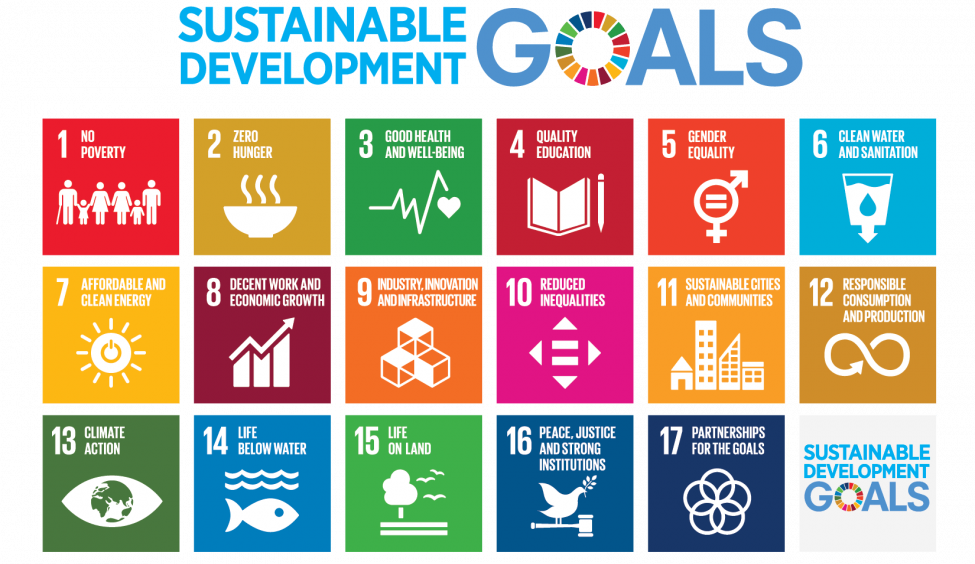
\includegraphics[scale=0.4]{SDGs.png}}
	\centering
	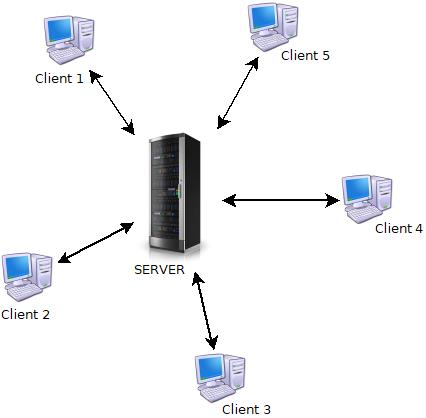
\includegraphics[width=2in]{CS_Arch1}
	\caption{Client Server System}
\end{figure}

The emerging Blockchain technology removes these pitfalls by laying a trust layer on top of the existing Internet technology. It replaces the mediator-centric model of information exchange with the peer-to-peer model or decentralized model of information exchange. It transforms the Internet into a trustworthy platform for doing business when transacting parties do not trust each other. It eliminates the role of mediator responsible for authenticating the identities of transacting parties.

\begin{longtable}{p{2.6cm}p{4cm}p{4cm}}
	\\ \hline
	~ & Client/Server Architecture & Decentralized Architecture \\ \hline \\
	Mode of Communication & Client Server communicate through each other via Internet protocols & {\em Peer to Peer} communication via internet protocols. \\
	Components & Nodes, Server, Communication Link & Nodes, Communication Link \\
	Architecture Style & Layered & Object-based \\
	Availability & Need to achieve high availability & No need to achieve high availability \\
	Servers & Only single server is present to serve client & Servers are distributed in system \\
	Privacy & It is easy to determine who is handling the content & Difficult to determine who is handling the content \\
	Failure & Bottleneck as the sever fails down & No bottleneck as services can be provided through other nodes \\
	Cost & Implementation cost is high & Implementation cost is negligible \\ \hline
	\\
	\caption{Difference Between Client/Server and Decentralized Architecture}
\end{longtable}

Initially emerged as a platform to exchange digital currency over the Internet, now the Blockchain technology gradually emerging as a general purpose platform for doing business over the Internet. Due to potential applications of Blockchain technology in various Fields, UN has included it as one of the frontier technologies to realize SDGs \cite{ftech}. 

This section provides an overview of basic elements of Blockchain and how it achieves the various quality attributes that make it as one of the promising technology. The Blockchain technology can be understood at conceptual level and at specific instance level. The Bitcoin, Ethereum, and Hyperledger are few common examples of specific Blockchain. This section, reviews the Blockchain technology at conceptual level. The four basic concepts common across the Blockchain implementation are: \cite{dinh2018}

\begin{enumerate}
 \item Distributed Ledger
 \item Cryptography
 \item Consensus Protocols
 \item Smart Contracts
\end{enumerate}

\subsection{Distributed Ledger} 

In a conventional sense, ledgers are the registers or log books employed for account or book-keeping operations. Similarly, in the context of a Blockchain based information system, ledgers are the databases storing up-to-date information about business transactions. These are distributed among all the nodes participating in the network. In a Blockchain environment, ledgers are not stored at a central place. They are distributed among all the nodes so multiple copies of a ledger exist in a business network or a community. Hence these are referred to as distributed ledgers. Whenever, a node in a network updates the ledger, all the copies of the ledger in the network are synchronized and they contain the same information.

These ledgers are used to store information about valuable assets. In the Bitcoin implementation, the first Blockchain based system, ledgers are used to store digital currencies. It may be used to store information about other valuable assets such as land records, diamonds, student's academic credentials and others.

\begin{figure}[h]
	%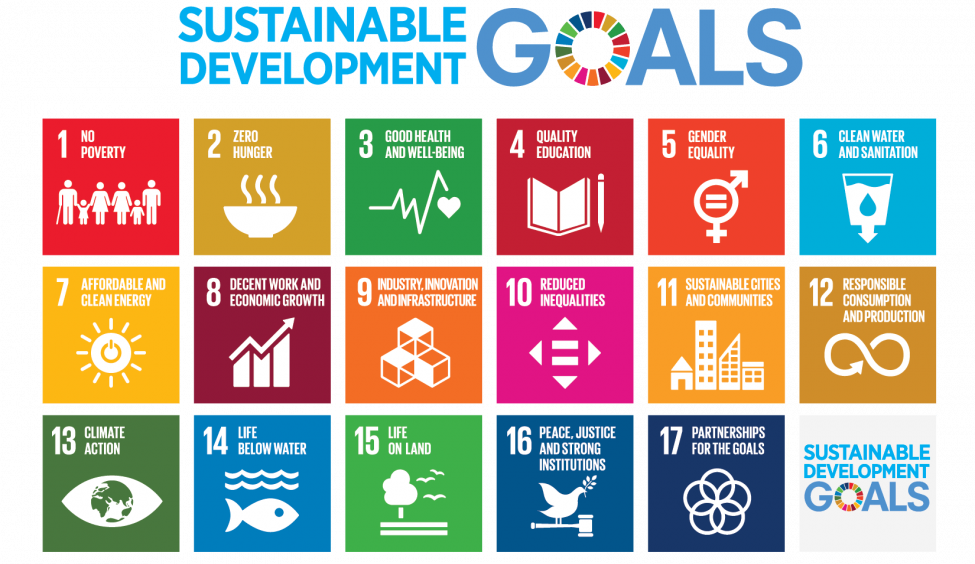
\includegraphics[scale=0.4]{SDGs.png}}
	\centering
	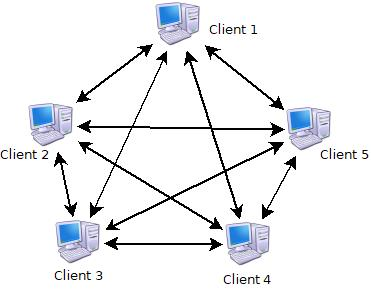
\includegraphics[width=2in]{Decentralise}
	\caption{Decentralized System}
\end{figure}

In a Blockchain-based information system, records in a distributed ledgers are arranged in a chain-format as shown in Figure \ref{bc} for storage purpose. Here, multiple transactions related to an asset are grouped in a block. The $n+1$th block in the chain links to the $n$th block and the $n$ block links to the $n-1$th block and so on. The first block in a chain is called a genesis block or the root block. Due to this peculiar storage arrangement the distributed ledgers are also known as Blockchain. Here it is worth to note that all Blockchain-based systems contain distributed ledgers but not all distributed ledgers employ Blockchain based storage mechanism. The Blockchain data structure permits only append of new records. Updating and deletion of records are not permissible.

The most important design feature of Blockchain based information system is use of hash pointers instead of physical memory based pointers to link blocks in a chain. A hash pointer is a message digest calculated from the information content of a block. When never a node attempts to tamper the information content, a small change in the information leads to ripple effect of changes in hash-pointers. Making it impossible to change the information once it has been recorded in the Blockchain. 

Facilitating mediator-less business transactions and supporting immutability of stored information are the two significant quality attributes associated to Blockchain based information systems. These qualify attributes are derived from replicating ledgers on all the nodes in a network and linking blocks in a chain through hash pointers.

Typically block chains are of two kinds based on how block chains are accessed i.e. private and public block chains. In a public Blockchain, any node can join and leave the network and validate the business transactions. While in case of private Blockchain the network is small and required permission to join and leave the network. Hence private Blockchains are also known as permissioned Blockchain and public Blockchain are known as permission-less Blockchain. For example, Bitcoin is a public Blockchain and Hyperledger is an example of private Blockchain.

 
\subsection{Cryptography}
Blockchain technology makes heavy use of cryptographic functions to assure trust among user community transacting over a Blockchain-based business network. A typical business network includes many un-trustworthy elements. In a conventional banking domain, an agent issuing the check without having sufficient balance in the account, or an agent forging a signature are typical examples. In a digitized economy, these challenges are aggravated because of information transfer over an unreliable communication medium. Hence, cryptographic functions, a set of mathematical functions, are used to encode messages to assure the security of information in a network containing malicious or un-trustworthy agents. These cryptographic functions address various purposes. Some of them are:

1) Authenticating identity of agents involved in a business transaction: Blockchain-based systems use a kind of asymmetric key cryptography. These protocols use two different keys called public and private keys, which are very large numbers. The public keys are open and used as addresses for performing business transactions while private keys are secret and used for validating the transactions. SHA-256 (e.g., Bitcoin) and ECDSA (e.g.,Hyperledger) are some of the cryptographic protocols used for this purpose. The private Blockchain use another service called membership service, which authenticates the identity for business transactions.

2) Ensuring Privacy: Maintaining the privacy of transactions is a challenge, especially in public blockchains (e.g., Bitcoin). In such systems, transactions are possible to trace to real-life identities. Advanced cryptography based techniques such as cryptographic mixers (e.g., Zerocoin) and Zero-Knowledge proof (e.g., Zerocash) have been found effective to address this challenge.

Cryptographic functions such as digital signature are also used to authenticate a particular transaction.

\subsection{Consensus Protocols}
In decentralized systems, agreeing upon the global state of the transaction is a challenge. In a centralized system, this is not an issue because only one copy of transaction history is present at the central authority (e.g. Banks main Server machine). Blockchain being a decentralized system holds multiple replicas of transactions at several nodes. Agreeing upon the unique state of the transaction is an issue which is solved by executing a consensus process involving all the nodes in the system. This process is typically carried out in three stages. In the first phase, a node is elected/selected as a leader node to decide upon a unique state. In the second stage, transactions are validated. In the third stage, transactions are committed. A variety of consensus algorithms exists in Blockchain based system. These are often compared based upon how scalable the algorithm is and a number of malicious nodes it tolerates. The Proof of Work (PoW) algorithm used in Bitcoin is one example of the consensus protocol. It selects the leader node responsible for deciding upon a global state by solving a cryptographic puzzle. It takes about 10 mins for solving the puzzle requiring large computational work and a lot of electric energy. It can work in the presence of 50\% malicious nodes in the network.
The Proof of Stake(PoS) is another consensus protocol in which a leader is selected with the highest stakes in the network. It has been found scalable as compared to PoW also works in the presence of 50\% malicious nodes in the network.

The Practical Byzantine Fault Tolerant (PBFT) is the third example consensus protocol which has been found scalable and works in the presence of 66\% (2/3) malicious nodes in the network.

\subsection{Smart Contracts}
Smart contract the most significant element in the Blockchain based system because it provides configuring the behavior of such systems. Blockchain programmers can customize the working of Blockchain systems by writing programs called {\em Smart Contract}. The smart contracts are scripts which are executed when a specific event occurs in a system. For example, in the context of Bitcoin, a coin may be released when more than one signatures are validated, or when miners solve a cryptographic puzzle.

These scripts can be written in a native language provided by Blockchain systems or general purpose programmable language. For example, Bitcoin provides a simple and less expressive native language to write a smart contract while Ethereum provides a Turing complete native language called Solidity to write smart contracts. In Hyperledger, Blockchain programmers can write a smart contract in general purpose language such as Java/Go.
 
\section{Sectoral Applications of Blockchain Technology}

\subsection{Blockchain Technology in Agriculture:}
Numerous business factors motivate the  adoption of Blockchain Technology in Agriculture sector. 

First and the topmost  key-factor behind the adoption of  Blockchain technology is to eliminate  bad  actors and poor processes involved in food supply chain. For example, {\em AgriDigital} ($agridigital.io$) is a cloud-based platform designed to provide efficient interface to agriculture supply chain.

Second key factor is to create trust among consumers and retailers about the originality and authenticity of food products.For example, $ripe.io$ is an organization which provides a Blockchain-based platform with this sole purpose.


Blockchain technology has potential to open up new market areas for food producers specifically farmers from the developing nations. For example, {\em AgriLedger} ($agriledger.io$) adopts the distributed ledger component of Blockchain technology to open up new market areas for the farmers.

 While designing such platform one of the challenge faced is \textit{mapping of physical commodity to digital}. For this, Internet of Things (IoT) techniques and various sensors are used to overcome such challenges. Second challenge was designing standards that certify the Blockchain technology is immutable and accurate. Also data fed to system is true. And last is poor Internet connection at the various places at the time of implementation of the system.

 .
The typical use-cases of blockchain technology in agriculture sector can be broadly classified as below:
\begin{enumerate}
    \item {\bf Blockchain for crowd-funding agricultural products} Entrepreneurs and  start-up organizations have been increasingly using blockchain as  crypto-currencies or  digitized tokens  to raise capital for their entrepreneurial ventures. This mode of application is generally known as Initial Coin Offerings (ICO) \cite{catalini2018initial}. 
    
    The ICOs are a type of digitized financial instruments which can be monetized through crypto-currencies or through fiat currencies.The $NagriCoin$ ($nagricoin.io$) is one such  application, which aims to raise capital to develop smart fertilizers stimulating plant growth. 
    
    \item {\bf Blockchain for agricultural supply chain management}  The use of blockchain technology for agricultural supply chain management is driven by various business factors.  First, paying the farmers their due share in food production is the key motivating factor behind the adoption of blockchain technology for food supply chain. The second most important factor is to address the  concerns about food safety in the minds of consumers. 
    
    For example, the $AgriDigital$ is a cloud-based supply chain management platform primarily supporting supply chain for grains. 
    
    The objective of such platforms is to effectively connect the various operators in the supply chain such as farmers, distributors, storage operators, retailers and consumers. 
    
    Creation of digital assets representing physical products, recording and tracking their flow within the supply chain are the main functionalities offered by  such platforms. They implement it by providing a set of smart-contracts executing over a blockchain implementation such as Ethereum.
    
  
    
    \item {\bf Tracking and Traceablity}
     Assuring about the quality of food-products and agricultural commodities is one of the main challenges faced by agriculture and food processing industries \cite{kamilaris2019rise}. Consumers expect authenticity about food products in terms of composition, origin, and purity.
    These expectations are valid when the food-products are costly, consumed at a distant place far from its origin and they are directly linked to the health and safety of consumers.
    
    Providing accurate and verifiable information  about the composition and origin of the food product is one of the solutions to address this challenge. The blockchain technology plays exactly this role while tracking and tracing the origin of food production.
    
    The blockchain-based solutions to address this problem are typically built around the immutability feature of the blockchain  along with other technologies such  as DNA marking, RFID tagging, QR coding, and isotape testing.
    
    \item {\bf Blockchain-based financial products for farmers}
    Conventional financial institutes such as banks, insurance companies and cooperative credit societies face the challenge of including small-farmers in the mainstream financial sectors. This situation leads to undue exploitation of farmers by illegal money lenders and traders.
    
    Blockchain as a technology initially emerged as a payment system through digital currencies (e.g. Bitcon) can be used to provide financial products specially designed for farmers.
    
   The $AgriWallet$ is one such example of saving scheme designed and implemented by COIN22 ($coin22.com$) for smallholder farmers to manage the risk  associated with droughts, floods and low-yield of crops. \cite{fao}
   
   Also the use of blockchain technology is currently being explored by any companies and government agencies to provide agriculture insurance, micro-credit and subsidy transfer. \cite{bermeo2018blockchain}
 
 
\end {enumerate}
	
\subsection{Blockchain for Financial Services:}

The  use of Blockchain in providing  financial services is motivated by the factors such as to eliminate the  role of mediators between  two transacting  parties,  to reduce  transaction time, and to simplify the transaction process. 

In such scenarios,  blockchain technology mainly plays the role of  validating  transactions. 
It helps to reduce the transaction charges by offering  efficient and secure way to transfer the funds either within a country or between two different countries. 

The use-case of blockchain technology in finical sectors belongs mainly to two categories. First in the area of payment and transfer and second record keeping and verification.

For example, the \textit{Mojaloop} is one of examples of the blockchain-based payment transfer platform developed for  Gates Foundation to connect financial service-providers and customers form all over the world. In addition to offering efficient payment mechanism,  blockchain technology  reduces the possibilities of  frauds such as corruption during disbursement of funds.  

Secondly, the features of blockchain technology such as distributed ledger and smart contracts have been used for effective aid distribution. Each steps involved during the aid distribution from donation to receipt of the amount are tracked and monitored using distributed ledgers. Donations are released upon meeting specific criteria and and occurrence of a pre-specified events encoded in the smart contracts. For example, $Amply$ \cite{bi} is a blockchain based protocol developed by IXO foundation which links  the release of Govt. subsidies to the attendance of children in a school.




Applications of blockchain technology in banking and finance sectors enables the attainment of  the  sustainable development goals  such as SDG1, SDG9, \& SDG8. For example,  World Food Program (WFP) used the blockchain technology to provide food-assistance to refugees from Syria.  
		
\subsection{Blockchain in Education:}

The information and communication technologies have revolutionized the
mode of delivering education. It has realized the goal of open education to all and created multiple ways to equip oneself and upgrade the skill set.
The blockchain technology is now providing  value added services in the education sector which includes credit transfer, issuing  transcript, digital certificates,  and payment for online courses. 

In the education sector, the uses of blockchain technology are categorized into following types.
\begin{enumerate}
    \item {\bf Record Verification and Validation} In this mode of use-case, blockchain is used as  distributed ledgers which  store and verify 
    academic credentials of students. For example, $BlockCert$ ($https://www.blockcerts.org/$) is a set of tools that provides functionality to create, store and validate blockchain-based digital certificates. 
    \item {\bf Information Sharing}When a student migrates from one university to another, universities need to share and transfer the academic credentials of a student. In this mode of application, blockchain technology enables effective transfer of academic information between two universities.  For example, the design of one such platform that enables credit transfer among institutes caleed $EduCTX$ is discussed in \cite{turkanovic2018eductx}.
    \item {\bf Identity Management} Online learners use multiple applications and services such as Coursera, Google Class Room, and  note taking apps (e.g., Keep). Securely sharing adnd authenticating identity credentials across the applications  remain a big challenge. Blockchain technology address this challenge by providing unique identifier accessible and verifiable across the applications. For example, $BlockStack$ ($https://blockstack.org/$) one such cloud-based identity management service.
    
    
These applications of blockchain technology are  realizing the goal of providing equal learning opportunities to every one i.e. (SDG-4)
\end{enumerate}



\subsection{Blockchain in Energy Sector:}
The energy sector worldwide is undergoing structural as well as functional changes. Decentralized network of renewable energy generators is gradually expanding which is currently dominated by the e conventional centralized grid structure. The functionalities of conventional power grid is also not only limited to the functions of  power generation and distribution but providing additional services suc as analyzing the data generated through deployment of smart devices and offering intelligent services to consumers.

The blockchain technology is the driving force behind all these changes. The features of blcokchain namely distributed ledger and smart contracts are being increasingly used to provide additional services. A comprehensive survey of such services is presented in \cite{andoni2019blockchain}. Some of these services are:

\begin{enumerate}
    \item {\bf Wholesale Energy Trading and Supply} The technologies such as distributed ledgers and smart contract is used to simplify the business processes involved energy trading and supply. In this context, blockchain technologies are primarily used as record keeping, autonomous agents executing business logic,and for payment and transfers. Elimination of intermediaries and reduced transaction times are the benefits gained by adopting blockchain-based approach.
    \item {\bf Imbalance Settlement} It is a process executed by grid operators which aims to remove discrepancies between energy units sold by energy suppliers and energy sold by distributors to the consumers. Blockchain technology provides efficient solution to this problem which normally take months for settlement. Here also, distributed ledgers are used to keep the track of energy generation and consumption.
    \item{\bf P2P Trading} Peer to Peer trading is form of trading in which energy providers or generators directly sells the energy units to consumers. Thus eliminating the role of energy distributors. Here blockchain technology is used as platform that facilitates energy trading in-exchange of digital currencies. 
\end{enumerate}

Providing affordable access to reliable and modern energy (SDG 7) is one of the sustainable goals that blockchain technology is realizing through above mentioned use-cases. Further blockchain technology is providing an effective platform for energy trading in micro-grids and community owned energy systems.

\subsection{Blockchain for E-Governance:}

Government agencies face the challenge of providing transparent and citizen-centric services. 
These agencies looking at blockchain technology as a medium to improve the quality of their service.
These agencies have been adopting blockchain for multiple application areas. Some of which are listed below:
\begin{enumerate}
    \item {\bf A Platform for offering unified services} The government of Estonia is using Blockchain as a platform to provide more than thousand services to its citizen. Here, the distributed ledgers are used to log and  audit each and every transaction of citizens with the government. The government of Estonia has issued digital-ID and signatures to all citizens for this purpose. The use of blockchain has brought transparency and trust in the services offered by the Estonian government.
    \item{\bf  E-voting} Democratic societies face the challenge of conducting free and fair elections. Conventional  ballot-paper based elections are prone to be rigged and manipulated. Blockchain technology is currently being explored as an alternative to address the challenge. The $Votem$ is a cloud-service that uses blockchain to securely caste votes by mobile or remote users. The system uses distributed ledger technology to record and verify the votes. 
    \item {\bf Land Records} Recording the information of land holding and ownership is one of the obvious usage of blockchain technology. The recording of such information in immutable registry and for archival purpose is essential to  avoid land-related frauds. In countries such as India and Sweden, the use of blockchain technology for land records has been initiated while in cities like Chicago the complete work-flow involved in land selling and buying is being automated through smart contracts.
\end{enumerate}

The use of blockchain technology in governance sector is directly assisting to to realize the goal of Peace, Justice, and Strong Institutions (SDG 16) and indirectly supporting the goal of equitable development (SDG 5).
 

\subsection{Applications of Blockchain in Environment and Climate Change}
Few applications of blockchain technology in area of environment protection and climate change has been envisioned.  Some of these novel applications include:
\begin{enumerate}
    \item {\bf Incentive Mechanism for Recycling Project} The blockchain technology is useful in rewarding digitized tokens or crypto-currencies for joining in recycling project. A digital token can be exchanged  for the deposit of plastic wastage.
     \item {\bf Enforcing Environmental Treaties} The feature of smart contract embedded in various blockchain platforms can be used to enforce environmental treaties executed by corporate agencies while carrying out developmental works.
     \item{\bf To implement Carbon Tax} The carbon footprint is a measure used for assessing carbon-dioxide emission caused by an individual, event or an organization. The blockchain technology is useful to track and record the carbon footprint and levy a tax based on carbon footprint or build a reputation system to provide incentives for low carbon footprint products and services.
    
\end{enumerate}

\subsection{Blockchain in Health Sector:}
The applications of blockchain technology in health sector belongs to following categories.
\begin{enumerate}
    \item {\bf Record keeping and ensuring confidentiality of information} The use of blockchain technology in health sector is driven by the motives to overcome the negligence of health related documents(e.g., medical prescriptions, and health reports) from patients side and to maintain privacy of health-care data. The health-care information is not only useful to an individual but in carrying out research related to genetic diseases.
    
    All such documents are valuable to medical researchers, health care providers, public health authorities and health insurance providers etc. 
    
    Blockchain technology provides a secure access to store existing  medical reports. These reports are made available on-demand through various Blockchain platforms. One of the applications is MedRec\cite{ekblaw2016case} is the used to store Electronic Medical Records (EMRs) on Blockchain. This information is accessible in a secure way to various  stakeholders such as medical researchers, and public health authorities etc. 
    
    \item{\bf Drug Supply Chain and Traceability}
    In the supply of drugs and medicinal products through pharmaceutical supply chain,  it needs to track the initial details of medical products while it is in transit. \textit{Modum.io} is the one of the European companies which implemented a hardware sensor to monitor temperature of drugs in pharmaceutical supply chain management. In such applications drug related information exchanged between drug manufacturers, wholesalers, pharmacist, and patient is recorded and tracked to authenticate the originality of the drug. 
    The features like distributed ledger and smart contract are used to implement these functionality.
\end{enumerate}

The combination of technologies such Artificial Intelligence, Blockchain and Internet of Things are providing various solutions and products to realize the goal of smart technologies for healthy life (SDG 3).

\section{Conclusion}


\bibliographystyle{vancouver-modified}
\bibliography{chapter}

\end{document}
